\documentclass[9pt,twocolumn,twoside]{gsajnl}
% Use the documentclass option 'lineno' to view line numbers

\articletype{inv} % article type
% {inv} Investigation
% {gs} Genomic Selection
% {goi} Genetics of Immunity
% {gos} Genetics of Sex
% {mp} Multiparental Populations


\title{Prostate Adenocarcinoma insights: Gene Expression approach from TCGA RNA-seq data}

\author[$\ast$,$\dagger$]{Adria Auladell-Martin}
\author[$\ast$,$\dagger$]{Joan Marti-Carreras}
\author[$\ast$,$\dagger$]{David Mas-Ponte}
\author[$\ast$,1]{Robert Castelo-Valdueza}

\affil[$\ast$]{M.Sc. in Bioinformatics at Department of Experimental and Health Sciences (CEXS), Universitat Pompeu Fabra}
\affil[$\dagger$]{Authors Contributed Equally to this work}

\keywords{prostate cancer; adenocarcinoma; RNA-Seq; paired data.}

\runningtitle{GENETICS} % For use in the footer

\correspondingauthor{Auladell-Martin}

\begin{abstract}
Transciptomics studies have improved substantially the molecular analysis of cancer, with the discovery of many new drug targets. The Cancer Genome Atlas Project has provided to the research society high quality RNA-seq data in many different tumor types. Prostate cancer, or prostate adenocarcinoma, is the second most deadly cancer disease, and one with the highest prevalences. The present article aims to perform an analysis of the differential expression and a functional analysis of RNA-seq data obtained from The Cancer Genome Atlas project. With previous sub-setting and normalization, a paired design of 42 tumor and 42 normal samples was used. Differential expression analysis was realized by multiple linear regression. Finally, a functional analysis was realized by hypergeometric test on gene ontology and gene set enrichment analysis/gene set variation analysis on various pathway datasets. A detailed analysis revealed that there is function enrichment in tumor samples when compared to normal samples. Differential gene expression seems to be less consistent than functional analysis, yet some can be linked to it. In the functional analysis appear pathways/GOs related to the tumorogenic processes: transporters and channels (SCN5A and CACNA1F), fatty acid pathways (GO:190157 fatty acid derivative transport), transcription factors (GO:0048710 regulation of astrocyte differentiation, EPHA8), between others.
\end{abstract}

\setboolean{displaycopyright}{true}

\begin{document}

\maketitle
\thispagestyle{firststyle}
\marginmark
\firstpagefootnote
\correspondingauthoraffiliation{adria.auladell@estudiant.upf.edu, joan.marti02@estudiant.upf.edu, david.mas@estudiant.upf.edu. Corresponding author: Robert Castelo Valdueza, robert.castelo@upf.edu.}
\vspace{-11pt}%

\section*{Introduction}

Prostate adenocarcinoma (PRAC), also referred as prostate cancer, is  the second most deadly cancer (following lung cancer), and one with the highest prevalence. As the American Cancer Society explains, about 1 man in 7 will be diagnosed with PRAC during his lifespan, and of those diagnosed, about 60\% are men over 65 years. Despite it might affect younger men (under 40 years old), this is not frequent. The mean of diagnosis is around 66 years old \citep{prostatestatistics}.

For patients whose cancer has spread, their survival time is usually one to three years. It was estimated that for 2011, 240,890 men would be diagnosed and 33,720 would die from prostate cancer. 

There has been multiple analysis of prostate cancer focused in RNA seq expression profiles \citep{rnaseq1,rnaseq2,zhai,rnaseq4}. \cite{rnaseq1} finded with a study of 14 profiles of prostate cancer multiple gene fusions, such as CTAGE5-KHDRBS3 and USP9Y-TTTY15, and a differential expression of long non-condign RNA in tumor samples. \cite{zhai} founded a low expression of Cullin-associated and neddulation-dissociated 1 (CAND1) and high expression of lincRNA in tumor samples.  But most of these studies were established with small cohorts, producing sometimes results not extrapolable to all the prostate cancer cases.

 The Cancer Genome Atlas Project (TCGA) \citep{tgca} is one of the most prominent international projects about cancer research in recent years and the availability of the data have been a key feature for scientist around the world to make a collaborative effort in order to analyze such amount of data. In the field of prostate cancer and as official publication, the authors of the Project have published a paper about the taxonomy of the cancer type \citep{Abeshouse2015}. In this study they have been able to detect the driver mutations in the samples and therefore classify the heterogeneity of the tumor in different molecular subtypes. 
 
\begin{itemize}
\item 74\% of all tumors being assignable to one of seven molecular classes based on distinct oncogenes drivers:
        fusions involving (1) ERG, (2) ETV1, (3) ETV4, or (4) FLI1 (46\%, 8\%, 4\%, and 1\%, respectively)
        mutations in (5) SPOP or (6) FOXA1; or (7) IDH1. (11\%, 3\%, and 1\%, respectively).
\item 25\% of the prostate cancers had a presumed actionable lesion in the PI3K or MAPK signalling pathways, and DNA repair genes were inactivated in 19\%.
\end{itemize}

But the main conclusions were established at genome level, without producing a deep analysis of the different RNA seq profiles decribed in the transcriptome assay provided by the project. For the presented reason we believe a differential expression Analysis is needed to fully understand the nature of this data and to proper interpret a common insight from different molecular tumor subtypes.  

The aim of this study is to analyse prostate adenocarcinoma RNA seq dataset provided publicly by TCGA in order to establish (1) differentially expressed genes (2) a functional analysis of this gene sets at individual level, gene ontology level and gene pathways level, and finally (3) an integration of the functional results in general prostate cancer traits. 

\section*{Materials and Methods}


The examination of the RNA counts can be performed in an average laptop. As a limiting factor for analysing the data, it is recommended to have at least 4 Gb of RAM and CPU Intel Core i5 or superior. HDD memory is not a limiting factor for this analysis.

\begin{figure*}[!h]
\centering

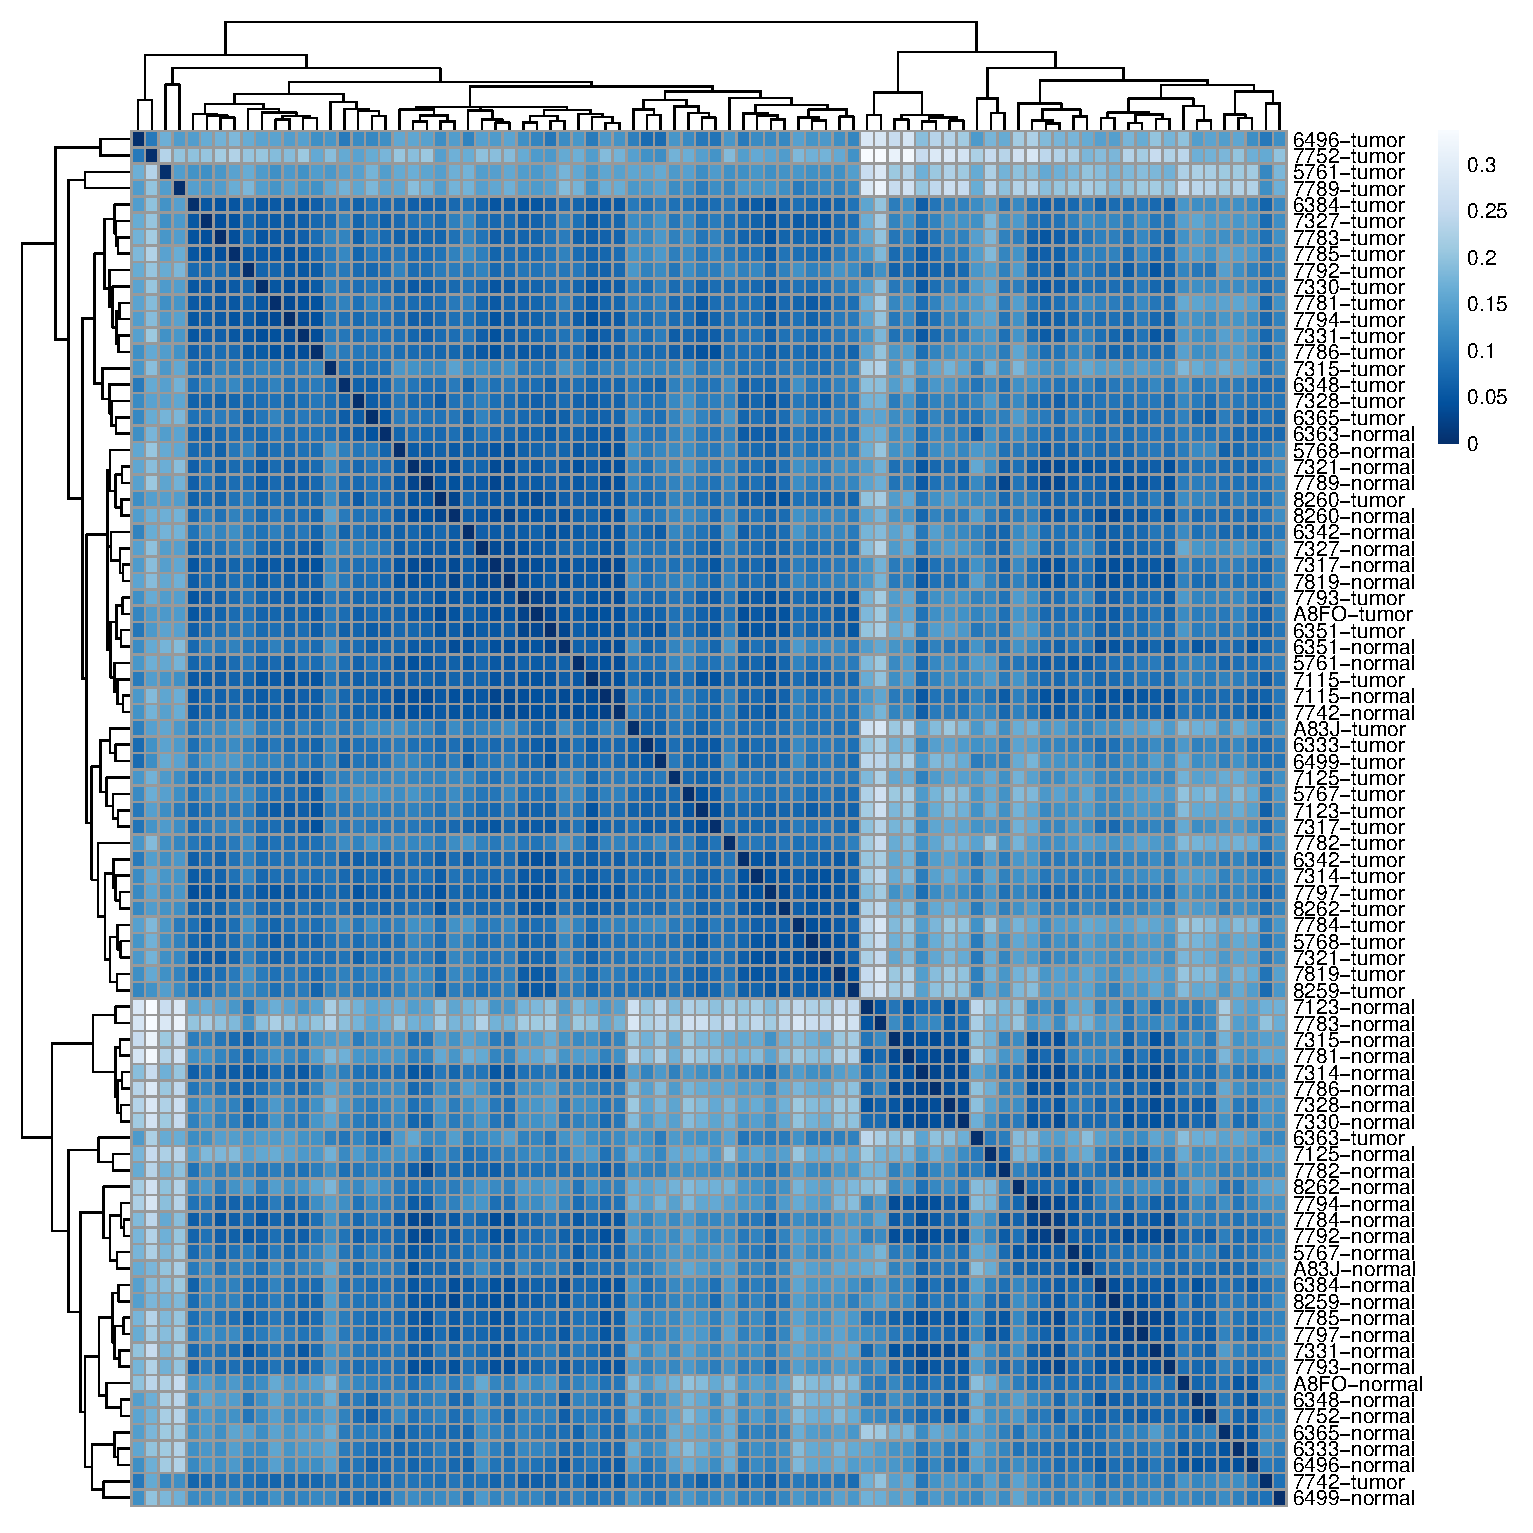
\includegraphics[width=.7\textwidth]{Clustering.eps}

\caption{Heatmap of sample-to-sample distances. After filtering and pruning our data set the image show the difference of all genes expression in logCPM units. The Clustering have been performed using a Spearman method. We can observe clearly 2 groups corresponding to tumor and normal samples. 
}
\label{fig:Clustering}
\end{figure*}

The software used was R version 3.3.0 "Supposedly Educational" \cite{R}. Main packages where download and installed through Bioconductor version 3.3 \citep{bioconductor}. Detailed information about package versions can be found on the section "Session Info" of the Supplementary Materials (SM).

In the following sections we describe briefly our analyses. However, a reproducible version of our analysis with all the code elements is also available in SM.


\subsection*{Data Availability}

The data sets are tables of RNA-seq counts generated by Rahman et al. \cite{Rahman15112015} from the TCGA raw sequence read data using the Rsubread/featureCounts pipeline for all data sets \cite{Rsubread}. The data was used for this analysis is a variation of the above mentioned datasets, curated by PhD. Robert Castelo-Valdueza. In the SM a link to the data is attached in order to download it. 

PRAC dataset consist initially of 502 tumor samples and 52 normal samples with clinical information of each sample. Library sizes of the samples presented different coverage, with values ranging from 20M reads per sample to even 90M.  The phenotypic variable that indicates the tumor or normal status of the sample is called type.  Considering that our analysis does not segregate for molecular subtype we already expect a big amount of variability that might be a caveat of our approach. However,it is possible that considering all the tumors we can get common insights from multiple subtypes of prostate cancer that can be also useful in future drug design studies. But for this reason the analysis will be realized in a subset of the complete dataset. 
\subsection*{Experimental Design}

The initial dataset presented 52 normal samples and 502 tumor samples. From this dataset, by patient barcode the dataset can be subsetted in a paired design of 50 normal and 50 tumoral samples and an unpaired design with 52 normal samples (with 50 form the paired design) and 452 tumor samples. It was decided that the paired design was a better choice, as this data presents almost no differences in the processement, suposing partially the elimination of possbile batch effects.

After applying the corresponding filterings (see SM), the dataset was composed by 50 normal samples and 50 tumor samples.

\subsection*{Quality Assessment and Normalization}

The dataset presented 20115 genes with expression data.  DGE functions were used for normalization, which belongs to edgeR package \cite{Robinson01012010}. Initially, normalization factors were calculated and counts per million reads (logCPM) computed. LogCPM distributions area were compared between normal samples and tumor samples. There were no significant differences, but a peak was observed below logCPM = 1. Since for these values the CPM the expression level we cannot establish real conclusions for those genes, transcripts with logCPM < 1 were deprecated. With this filtering, the number of genes analysed was reduced to 11722 genes. 

When plotting the log ratio - mean average plots (MA-plots) for all samples, it was noticed that the normalization procedure succeeded. There were no significant deviation of the samples, and the analysis proceeded without any other filtering.

\subsection*{Batch Effect Identification}

Batch effect was evaluated by means of the TCGA barcode information. The code specified center of analysis, tissue source site and plate of the NGS machine. The center was the University of North Carolina for all samples and the tissue source site/plate variables were equilibrated in the tumor/normal comparison (see SM).

To evaluate possible anomalous samples, hierarchical clustering (HC) from \cite{pheatmap} package and multidimensional scaling (MDS) from \cite{limma} package were performed. HC, clustered by Spearman correlation, presented mainly a good clustering, with some of the paired samples clustering together due to the similarities within individual (see SM). MDS plot presented an anomalous clustering of normal samples from the same batch. These samples were filtered out, remaining 42 tumor and 42 normal samples.


\subsection*{Differential Expression Analysis}

A design matrix was built with sample type (tumor/normal). LogCPM measurements were corrected with the  voom (mean-variance relationship of the log-counts) function present in limma package \cite{voom}. As a covariates,  patient barcode and surrogate variables inferred by SVA analysis were included. Surrogate variables are covariates constructed directly from high-dimensional data that can be used in subsequent analyses to adjust for unknown, unmodeled, or latent sources of noise analysis \cite{GSVA}.

With the design matrix and voom logCPM values, Multiple linear regression (MLR) was performed with \cite{limma} package. From MLR analysis, t statistics, moderated F-statistics and  log-odds ratios were calculated with empirical Bayes statistics from \cite{limma} package. P-values were adjusted with FDR measurements and cut-off was established at genes presenting 1\% of FDR. To evaluate results p-values and moderated t-statistics were plotted and DE genes were visualized in volcano plots and  MA plots  from \cite{limma} package (see SM). Top DE hits were visualized with Gviz package.


\subsection*{Functional Enrichment}

The resulting DE genes from the previous analyses have been tested for functional enrichment using Gene Ontology gene sets. A hyper-geometrical test from the GOstats package \cite{GOstats} was used. As parameters, a p-value cut-off of 0.01 have been set in order to filter only the most significant results. Then, the results have been pruned again for sets with at least 8 genes to avoid extreme results with infinite OddsRatio.

The same analysis have been also performed in the DE over-expressed and under-expressed gene lists to clarify if the GO biological process is indeed enhanced or decreased in tumor cells. The aim of this stratified analysis is to improve the biological content of our results.


\subsection*{Gene Set Expression Analysis}
In order to analyse differential expression in gene sets and not uniquely at the gene level 2 different approaches have been used, a Gene Set Enrichment Analysis (GSEA) and a Gene Set Variation Analysis (GSVA).


For both GSEA and GSVA the gene sets from the GSVAdata package \cite{GSVAdata} have been selected. After that, the original gene sets were reduced only to curated gene sets  (C2 type) . In this case the KEGG  \cite{kanehisa2016kegg}, Reactome \cite{fabregat2016reactome} and   Biocarta \cite{nishimura2001biocarta} databases were selected. Gene Sets related with Prostate Cancer have been also included from the same data package.


The package GSEABase \cite{GSEABase} was used to define Gene Sets and match gene identifiers to our Entrez Id codes. The classic GSEA consist in the generation of an incidence matrix that let us build a Enrichment Score by that is dependent on how many genes from the gene set are ranked as most DE genes. It is also an enrichment approach, however, it uses the expression values from the expressed genes to rank them so therefore it is been using expression data.

The GSVA package \cite{GSVA} was used to define the set expression values. Then, limma  \cite{limma} and SVA packages were used to perform the linear regression and to improve the model respectively \cite{leek2007capturing,svamanual} . Finally, the 30 top DE pathways have been clustered by sample in order to obtain a clear visualization of the ones over and under-expressed in tumor and normal samples.


\section*{Results}
\subsubsection*{Differential Expression Analysis}

\begin{figure*}[!h]
\centering
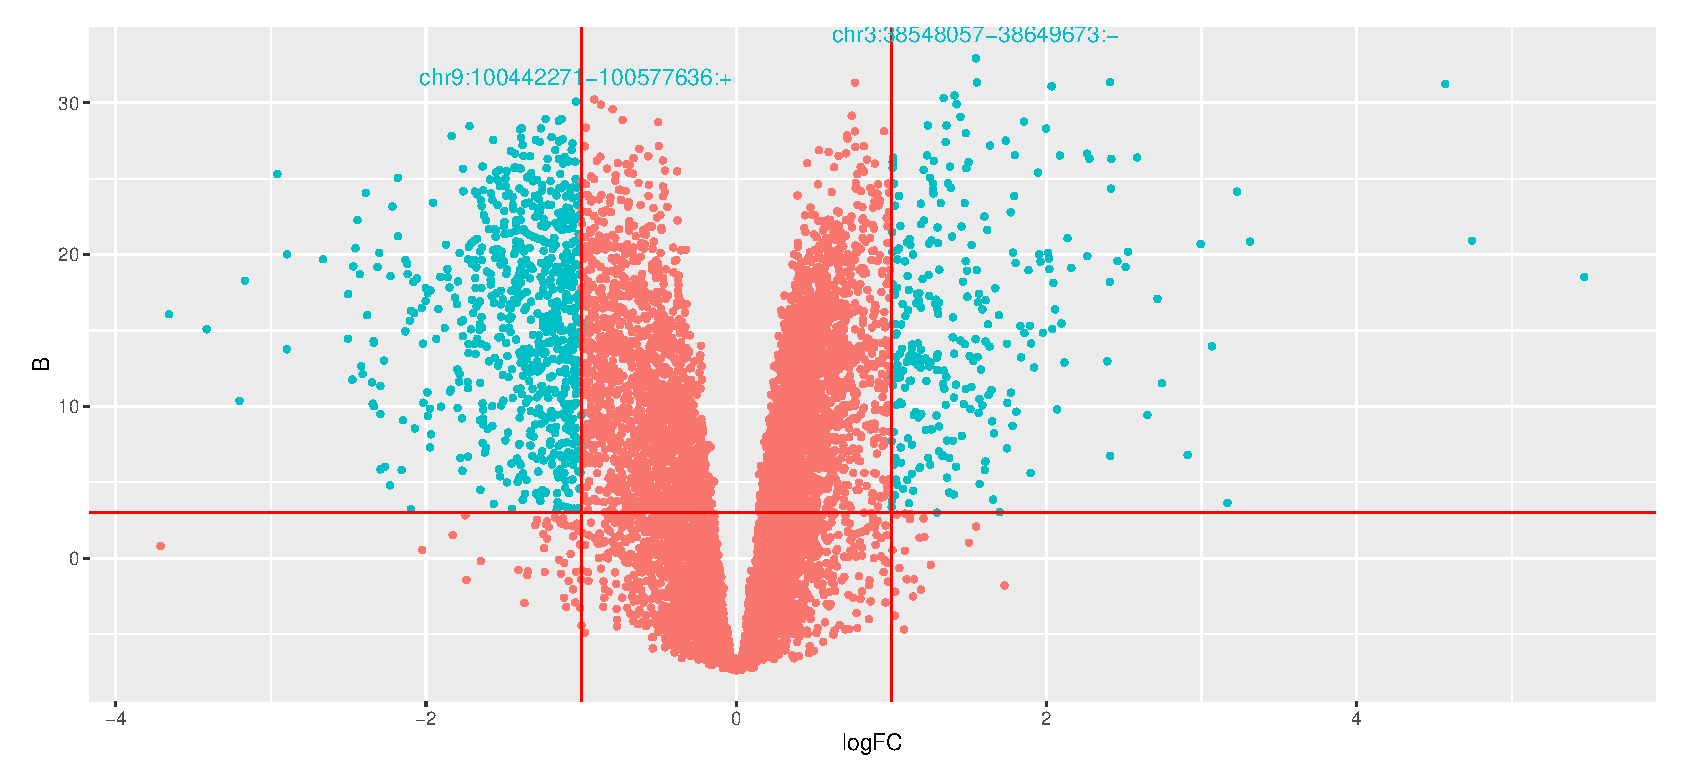
\includegraphics[width=\linewidth]{Volcano.eps}
\caption{Volcano plot representing the DE genes (over-expressed) in the right side and under-expressed in the left side. Axis represent intensity, logFC (2-fold expressed genes) at X-axis, and significance, B (derived from FDRCutoof = 0.001) at Y-axis. Crossing lines represent the threshold by which genes have been minimally accepted. Blue dots are accepted transcripts, red dots are rejected. Most scoring genes are highlighted.
}

\label{fig:volcano}
\end{figure*}

After computing the multiple linear model test, and the eBayes test \cite{limma} 	it was found out that:

\begin{itemize}
\item 2168 genes are under-expressed in tumor samples compared to normal samples.
\item 7569 genes have no significant difference in their expression between sample types.
\item 2127 genes are over-expressed in tumor samples compared to normal samples.
\end{itemize}

Volcano plot (Fig. \ref{fig:volcano}) was performed to graphically represent the distribution of genes by its B (signification) and its log fold changes (intensity). Despite that there are lots of genes that fall out of the rejection zones, in fact they conform a gradient of signification and only the topmost 5 will be taken into account for the rest of the article, as it is more likely that their values are worth. These 5 genes were then searched using the UCSC browser, using the RefSeq track, as it is more up-to-date (see supplementary material).

\begin{itemize}
\item chr1:225 codifies for \href{http://www.genecards.org/cgi-bin/carddisp.pl?gene=EPHA8}{EPHA8} which is an ephrin receptor, a neuronal factor.
\item chr2:101 codifies for \href{http://www.genecards.org/cgi-bin/carddisp.pl?gene=SNORD89}{SNORD89} which is a small nucleolar RNA.
\item chr3:385 codifies for \href{http://www.genecards.org/cgi-bin/carddisp.pl?gene=SCN5A}{SCN5A} which is a sodium channel voltage gated V Type.
\item chr11:11 codifies for \href{http://www.ensembl.org/Homo_sapiens/Gene/Summary?g=ENSG00000255292;r=11:112086903-112193805}{AP002884.2} which seems to mitocondrial protein (but does not appear on RefSeq).
\item chrX:492 codifies \href{http://www.genecards.org/cgi-bin/carddisp.pl?gene=CACNA1F}{CACNA1F} which is a calcium channel voltage dependant L type.
\end{itemize}

EPHA8 is a prognosis marker for cancer (malignant marker). It appears over-expressed in several tumor types, between them prostate cancer \cite{proteinatlas,uhlen2015tissue}.

SNORD89 is related with several cancer-related pathways:  anaplastic large cell lymphomas, lymphoma (NHL) cell lines, metastasis and death cell in colon cancer, prostate cancer, ovarian adenocarcinomas, etc \cite{tcng}.

SCN5A is a voltage-gated sodium channel (VGSC), a group that is known to be related with metastatic potential of breast cancer, prostate cancer and lung cancer between others \cite{Nelson2015}.

AP002884.2 seems to be an unmapped transcript. A more accurated display of the region, reveal that AP002884.2 compromises 2 genes SDHD-006 and BCO2-009. SDHD-006 is the 6th subunit of the succinate dehydrogenase, which is known to play a role as oncometabolite \cite{oncometabolites} and BCO2-009 is related with the synthesis of vitamin A through oxidation of carotenoids  and beta-carotene and have and strong relation with all kinds of cancer \cite{proteinatlas,uhlen2015tissue}.

We suggest that in the case of AP002884.2 there has been an error in the mapping phase of the reads. We have considered to take into account both proteins (SDHD-006 and BCO2-009) has both can be traced to carcinogenic processes.

CACNA1F is related with several cancers like colon cancer, breast cancer, melanoma, myeloma and prostate cancer \citep{tcng}.


It can be concluded, thus, that the main over-expressed genes in tumor samples are those related with signalling, metabolism and transcription modulation; fields that are usually related to carcinogenic processes.


\subsubsection*{Functional Enrichment}

From the 11143 gene ontology (GO) biological processes (BP) terms tested, only 21 presented significant results (p < 0.01). The top 5 results in odds ratio decreasing order are listed in Table \ref{tab:GOenrichment}.

The first result is related with processes that modulate the frequency, rate or extent of astrocyte differentiation (GO:0048710). This result coincides with other studies provided by \cite{neuroendocrine3, neuroendocrine2} and the review realized by \cite{neuroendocrine1}. Some of the set genes haven been described in other studies as neurodifferentiaton markers, such as EPHA4 \cite{neuroendocrine_EPA}, SEPRINE2 \cite{mckee2013protease} and others.

Response to vitamin A is a unexpected result: it is well known in prostate cancer the relationship with vitamin D \citep{vitamin0,vitamind1,vitamind2,vitamind3}, but little is known of the relationship with vitamin A. \cite{vitamina1} described a correlation between lack of vitamin A and prostate cancer, but there is no much other analysis in the field. Also, \cite{vitamina2} studied the relationship between vitamin A and apoptosis in prostate cancer, relating indirectly some of the genes such as retinoic acid receptor-beta (RARA), whose expression could be downregulated in cancer.

Both icosanoid secretion and fatty acid transport have been related with cancer \citep{fat1,fat2}. Eicosanoid are biological lipid molecules that are implicated in pathological processes. Being part of the  cyclooxygenase (COX) and lipoxygenase (LOX) pathways, they present mediator effect in the proliferation of cancerous cells and regulate tumor vascularization \citep{fatvascu} As we can see, the gene sets are almost identical, with SLCO2A1 present as a difference in fatty acid transport.

Finally, hystone acetylation (HA) presents relationship with cancer due to the regulatory role during transcription of genes through its influence on chromatin conformation \citep{histoneacet, histoneacet2, histoneacet3, histoneacet4}. Since in GO studies we only evaluate DE gene sets, this gene ontology factor can be related with the normal type. This would coincide with the expectation, since HA supresses tumor formation \cite{histonea}.


One consideration about the Gene Ontology analysis using hypergeometric tests is the variation of results with the parametic adjustment of the researcher. P-value cut-off and minimal gene sizes change the results of the functional enrichment analysis considerably. This makes the assay subjective for each researcher parametic decisions. With that purpose in mind, our analysis was restrictive to an small specific subset of GO terms, losing some other authentic results but reassuring the ones obtained.



\begin{table*}[!h]
\centering
\caption{Gene Ontology enriched terms. Columns present the GO identificator (GOBPID), the associated pvalue, odds ratio magnitude of the result, the Expected count of random hits (ExpCount), actual count (Count), size of the gene set (Size), a brief description (Term) and the hit genes. }
\begin{tableminipage}{\textwidth}
\small
 \begin{tabular}{|l|c|r|r|r|r|r|p{3.4cm}|p{5cm}|}
  \hline
 & GOBPID & Pvalue & OddsRatio & ExpCount & Count & Size & Term & Genes \\
  \hline
 1 & GO:0048710 & 0.00 & 11.20 & 7.53 &  13 &  14 & regulation of astrocyte differentiation & DAB1, EPHA4, F2, FGFR3, ATF5, PRPF19, BIN1, HES1, IL1B, NTRK3, SERPINE2, CNTN2, NR2E1 \\
   2 & GO:0033189 & 0.01 & 9.47 & 6.45 &  11 &  12 & response to vitamin A & DNMT3A, DNMT3B, GATA4, ARG1, LTC4S, RARA, RXRA, TSHB, TYMS, CAT, ALDH1A2 \\
   3 & GO:0032309 & 0.01 & 6.03 & 8.60 &  14 &  16 & icosanoid secretion & ABCC4, ACE, DRD3, AGTR2, ACSL4, ANXA1, IL1B, NTSR1, OXT, P2RX7, BDKRB2, SYK, CYP4F2, TNFSF11 \\
   4 & GO:1901571 & 0.01 & 4.31 & 9.68 &  15 &  18 & fatty acid derivative transport & ABCC4, ACE, DRD3, AGTR2, ACSL4, ANXA1, IL1B, NTSR1, OXT, P2RX7, BDKRB2, SLCO2A1, SYK, CYP4F2, TNFSF11 \\
   5 & GO:0043966 & 0.01 & 3.45 & 13.45 &  20 &  25 & histone H3 acetylation & TRIM16, TAF6L, WDR5, CHEK1, KAT7, SGF29, DR1, BRD4, KAT6B, WBP2, SIN3A, BRPF3, PER1, PIH1D1, CSRP2BP, BRCA2, TAF10, BRPF1, KAT2B, SUPT7L \\
   \hline
 \end{tabular}
 \label{tab:GOenrichment}
\end{tableminipage}
\end{table*}



\begin{table*}[!h]
\centering
\caption{\bf Gene Set Enrichment Analysis terms. Columns present the Gene set names, the relative tumor expression (with relation to cancer samples), its Z-value (score used to rank them) and the genes that are related with it.}
\begin{tableminipage}{\textwidth}
\small
\begin{tabular}{|l|c|c|p{6.3cm}|}
 \hline
Gene Set & Relative tumor expression &  Z-value & Genes \\
  \hline
REACTOME DEADENYLATION OF MRNA & Over-Expressed  & 19.19 & EIF4A1, EIF4A2, EIF4B, EIF4E, EIF4G1, CNOT2, CNOT4, RQCD1, CNOT8, PAN2, CNOT1, CNOT10, PABPC1, CNOT7, CNOT6, TNKS1BP1, CNOT6L, PAN3 \\
REACTOME SMOOTH MUSCLE CONTRACTION & Under-Expressed & 18.70 & ACTA2, ACTG2, CALM1, CALM3, ITGA1, ITGB5, PXN, TPM2, VCL, SORBS1 \\
REACTOME BOTULINUM NEUROTOXICITY & Over-Expressed &  17.62 & SNAP25, SYT1, STX16, STX11, STX10, STX6, STX12, STX1B \\
REACTOME ENDOGENOUS STEROLS & Under-Expressed & 17.54 & CYP8B1, CYP11B1, CYP51A1, CYP46A1, CYP39A1 \\
\hline
\end{tabular}
\label{tab:GSEAenrichment}
\end{tableminipage}
\end{table*}


\subsubsection*{Gene set expression analysis}



\begin{figure*}[!h]
\centering
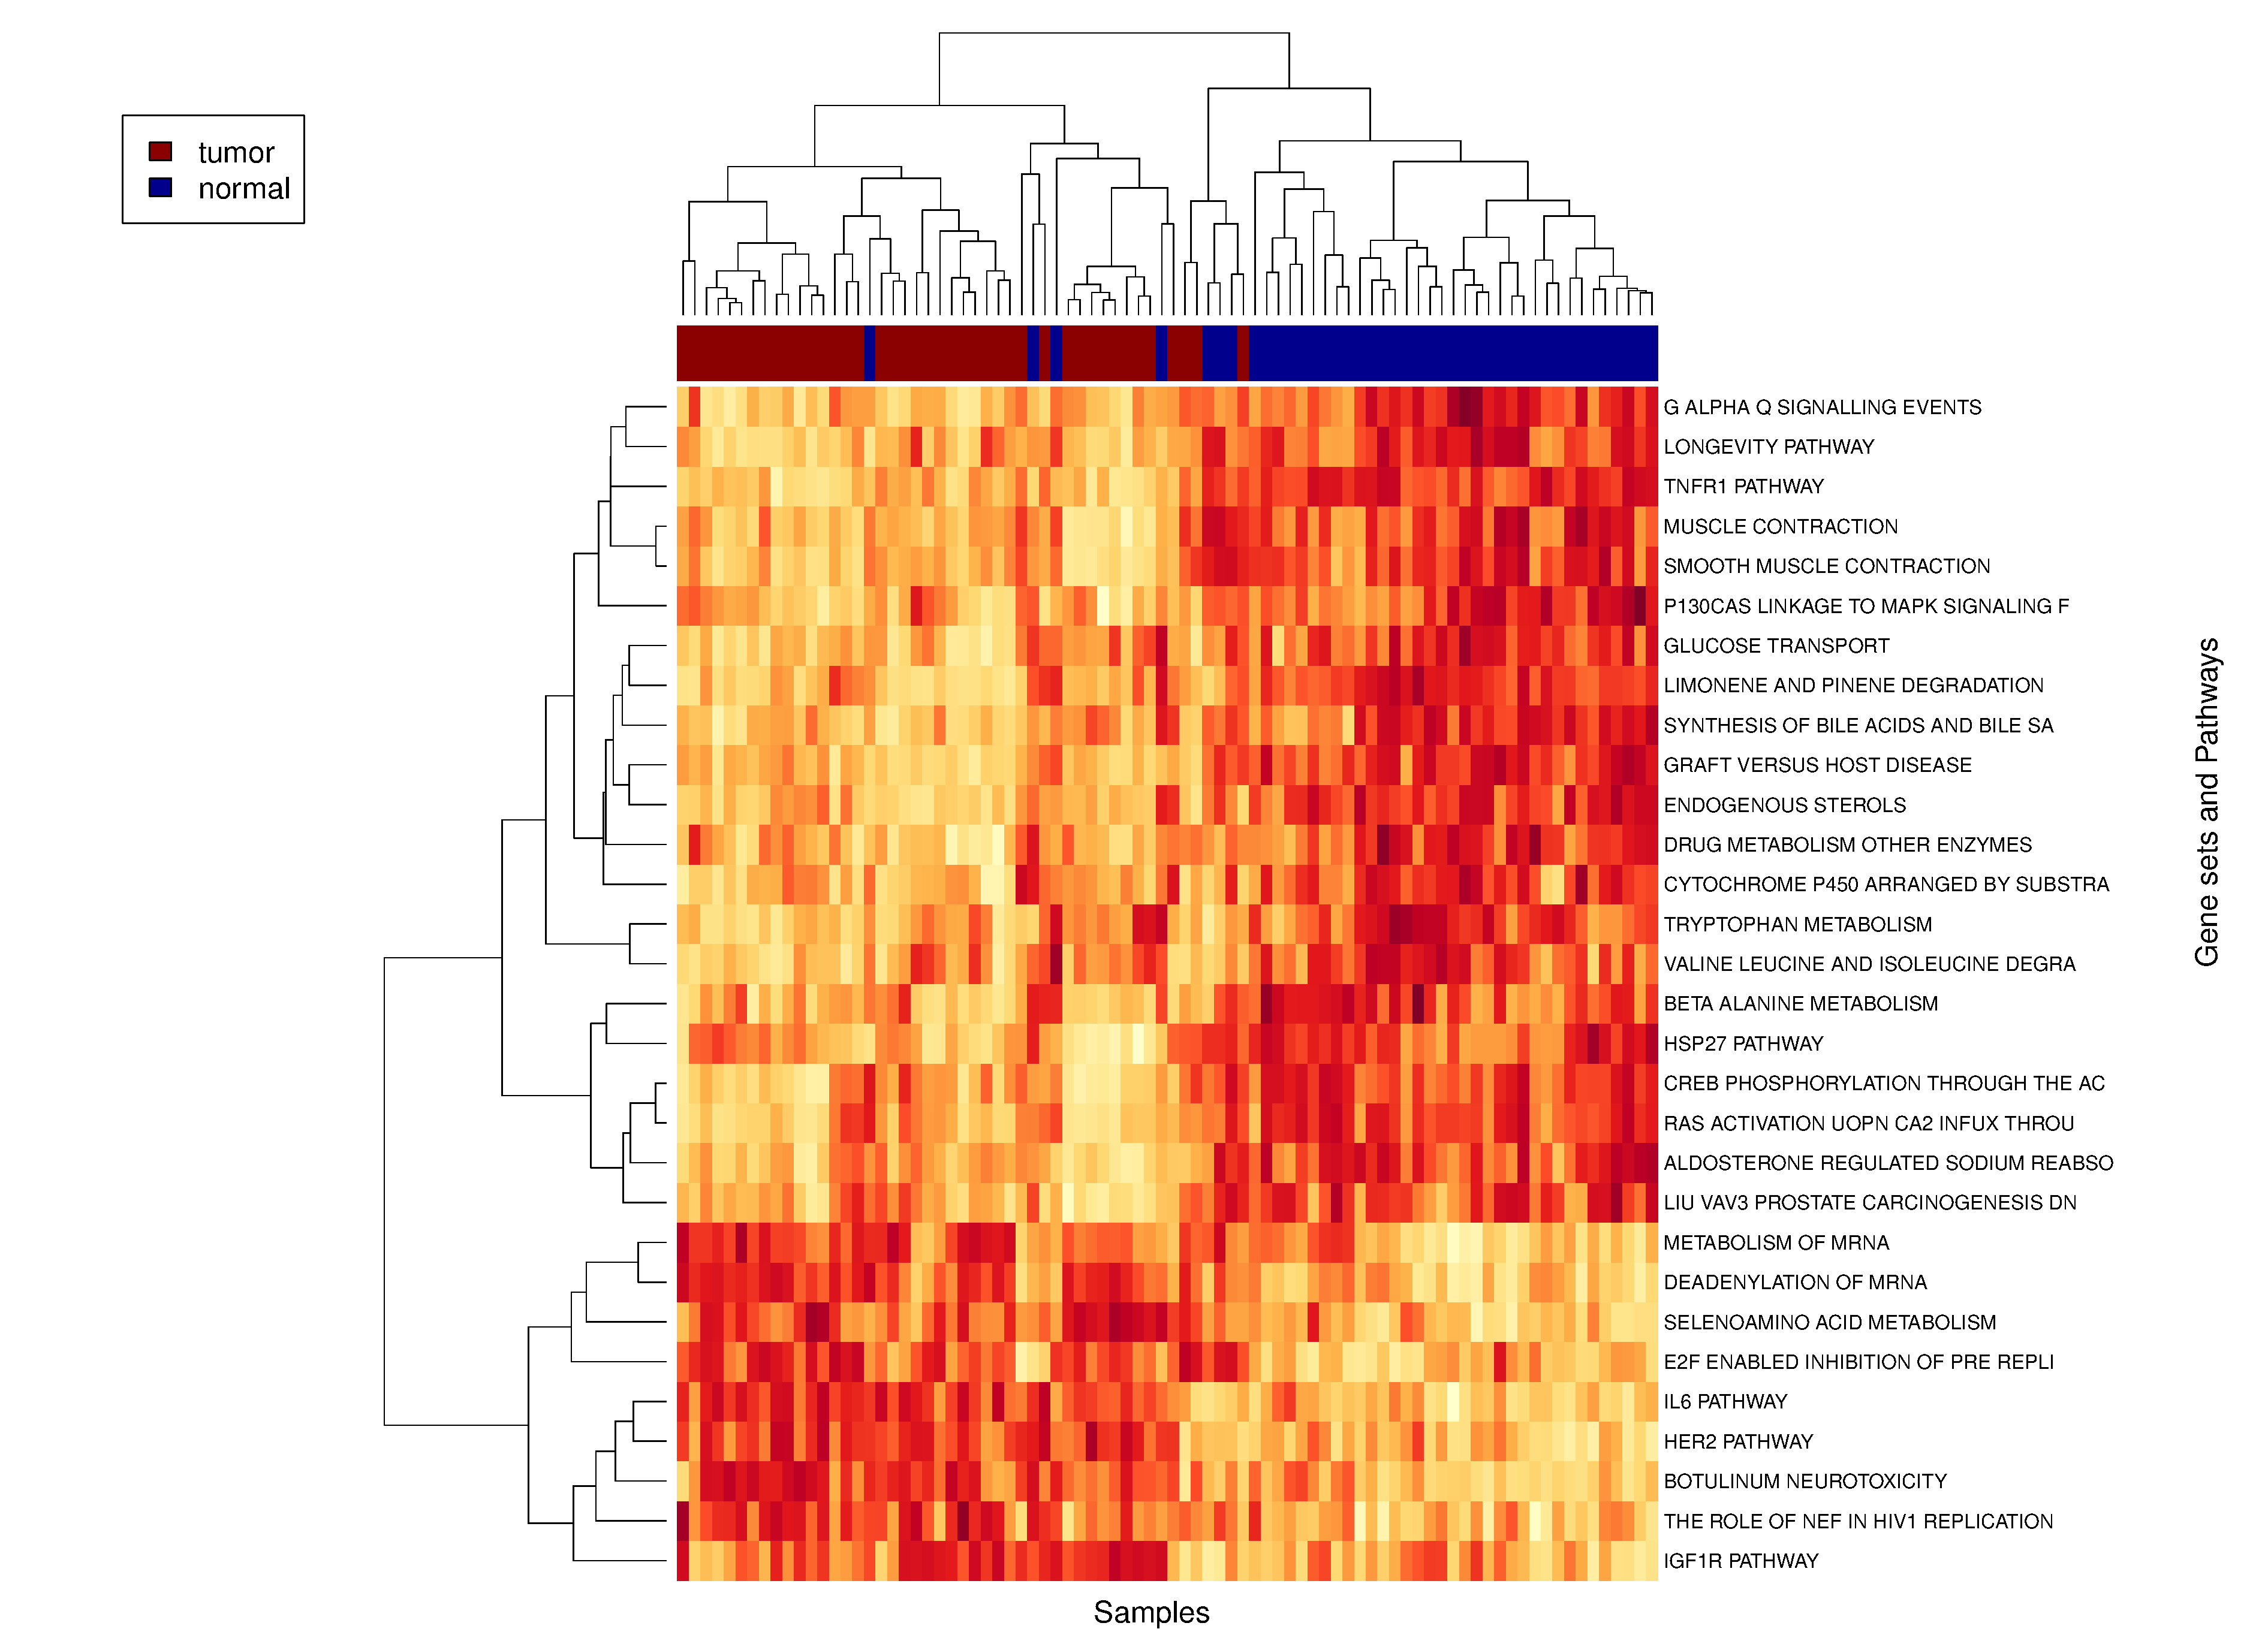
\includegraphics[width=1\textwidth]{ClusteringGSVA.eps}
\caption{Heatmap from the Clustering of the DE gene sets obtained from GSVA and samples.  Sample clustering has been performed using a Spearman method with the values of the differentially expressed genes. The two types are clearly differentiated. Heatmap of the pathways and gene sets is presented, clearly differentiating the two populations. }
\label{fig:ClusteringGSVA}
\end{figure*}


As mentioned above, 2 approaches have been used to detect Differential Expression at gene set level. The results from the enrichment approach are in table \ref{tab:GSEAenrichment} meanwhile the results from the Variation approach are shown in figure \ref{fig:ClusteringGSVA}.

In the first approach (table \ref{tab:GSEAenrichment}), the top ranked gene set differential expressed is the deanylation of mRNA which is a gene set related to the maturation of transcribed RNA. They are mostly expressed ubiquitously among the human tissues as they play a basic role in protein synthesis. From the selected genes, 4 families sum up their function. EIF4 and CNOT have a role as transcriptional regulators as they are part of the protein complex involved in this process. PAN in the other hand is important in the stabilitation of the mRNA and participates in the binding to the polyA tail. Finally, the TNKS1BP1 is a gene reported as key in nuclear stability of genome and have also been related to participate in the p53 pathway, which is a clear tumorsupresor. This pathway presents a small over-expression that may indicate a higher rate of protein transcription activity in cancer cells \cite{proteinatlas,uhlen2015tissue}.

The next gene set in the top ranked DE is the muscle contraction, also from the reactome database. This pathway is expressed mostly in the muscle tissue but it also presents expression in the urinary bladder, the gastrointestinal track and the prostate \cite{proteinatlas,uhlen2015tissue}. Its genes code for cytoskeletic related proteins like Actin, Calmodulin and Integrins that are key proteins in the cell shape determination. An under-expression of this pathway could easily be related with a undifferentiation of the cancer cells through the Epithelial–mesenchymal transition (EMT) \citep{yilmaz2009emt}.

The top3 and top5 hits from the GSEA are in fact related. Although the Botylium Toxicity pathway has some brain specific genes (SNAP25 and SYT1) and this seems to be unrelated with prostate and with cancer, the other genes in the set are expressed ubiquitously among the human body. These genes are related with the SNARE vessels and are also detected in the top5 gene set from the KEGG database \textit{SNARE INTERACTIONS IN VESICULAR TRANSPORT} as seen in the supplementary material report. SNAREs have been widely reported as tumorogenesis genes due to their control in multiple signalling and transportation pathways.

Finally, the top4 gene set detected, Endogenous Sterols is a gene formed by the CYtochrome P450 family that is key in the clorestherol homeostasis. There are genes responsible for its biosynthesis like CYP8B1 and from its degradation and conversion to bile salts like CYP39A1. This production of bile salts is also found to be related with prostate cancer in our following analysis, GSVA. The different genes in the set are expressed in a range of hormone secretory organs. Moreover, Prostate Cancer has been associated as a cholesterol dependent cancer and the cholesterol levels in blood are associated with bad prognosis \cite{krycer2013cholesterol}. This can be explained as cholesterol is a key molecule to  maintain the structure of the cell membrane and it is a important component of the lipid-rafts involved in signal transduction.


The top30 results from the Variation approach can be summed up in the figure \ref{fig:ClusteringGSVA} with a heat map that cluster the different gene sets in weather over-expressed or under-expressed in Prostate Cancer. The volcano plot regarding their significance is shown in the supplementary material. In the volcano plot is clear how the under-expressed side of the plot is more noisy (and more significant) than the over-expressed.

As first observation is clear the overlap between the GSVA and the GSEA that from their significant predictions we get an 74\% of overlap in their hits (see supplementary material). We can also get a similar idea from the selected top30 where already reported gene sets are significant also in this analysis. For instance, the mRNA deanylation and the SNAREs pathways are found also over-expressed in tumor cells. The deregulation of cholesterol levels and the dedifferentiation via under-expression of actins and integrins can be also seen in this analysis.

As a new hits we can get some interesting results in both sides of the expression. The HER2 pathway is strongly related with other cancers like Breast Cancer but have also been associated to prostate cancer by \cite{yeh1999her2} and its the most clear hit in our GSVA. Our top2 hit is the interleukine related gene set that would imply the inflamation of the cancer tissue. A role for IL-6 in prostate cancer has also been reported \citep{chung1999characterization}.

In the over-expression hits can still be found other growth factors like the Insulin-like growth factor, also reported in \cite{hellawell2002expression}, or the cell cycle regulator E2F gene set that some studies have used as target to unresponsive prostate tumors to androgen-deprivation therapy \citep{kaseb2007androgen}.

In the top part of the heat-map there are also new hits reported from the GSVA. The  \textit{VAV3 PROSTATE CARCINOGENESIS DN} \citep{liu2008targeted} is a gene set from Reactome that contain downregulated genes in a specific prostate cancer type characterized by the over-expression of VAV3. The Hsp27 gene code for a heat-shock protein that could be related with the heat response GO biological process found also in the GO enrichment analysis with FDR cutoff of 0.05 (data not shown).


\section*{Conclusions}

As a general conclusion we have to remark the amount of variability we had to deal with among the different steps of our analysis. This have let us to obtain several DE genes with a no clear pattern. We believe the main source of this variability may be due to different molecular sub-types as reported by the original TGCA paper \citep{Abeshouse2015} mixed up in our analyses.  As further research, it would be a good approach to analyse the DE of genes and gene sets in different sub-types independently to get unique expression patterns per sub-type. In addition, despite the fact that a volcano plot describes the most differential expressed genes, maybe it is not as relevant or important as the clustering methods or the GSVA methodology for the intention of this report.
 

Our study have a wide and comprehensive approach so we have tried to extract with different analysis the so called hallmarks of cancer in our samples. The hallmarks of cancer are well known biological capabilities that a tumor acquire during a multi-step development. Right now, the cancer field considers about 10 different hallmarks, sustaining proliferative signalling
evading growth suppressors, resisting cell death, enabling replicative immortality, inducing angiogenesis, activating invasion and metastasis, reprogramming of energy metabolism, generating genome instability,  evading immune destruction and promoting inflammation\citep{hanahan2011hallmarks}. In our study we had samples from several hallmarks coming from different analyses. We detected several proliferative signals like the HER2 pathway and the Insulin-like groth factor. We can also see the Interleukine-6 pathway also over-expressed in tumors that may be related with promoting inflammation in the tumor region. The EMT or activation of metastasis can be also observed in the deregulation of the cytoskeleton proteins and the deregulation of cholesterol homoeostasis. We find some change in expression in the glucose transporter pathway that would be related with the metabolic hallmark. The immortality and the lack of stability in genome can be related with some of the nuclear genes like the SNORD89 detected in the classic DEA and the TNKS1BP1 gene that is clear related with the genome stability. 

Moreover, we can extract other conclusions. We have detected some calcium dependent pathways and proteins that could be related somehow in an abnormal signal transduction leading to a cancer progression. It is also remarkable how the homoeostasis of sterols and fatty acids have been selected in the different analysis and could be related with the change of shape. Finally we find remarkable the link between several neuronal genes and our cancer samples. They could actually be a artifact, however, a lot of SNARE genes are highly related with neurons signalling pathways that would participate in prostate cancer. 

As a final remark, we think further investigation is needed in following a cancer sub-type approach more than the usual studies. If we could distinguish not only cancer sub-types but also cancer sub-populations in our samples the variability related to the expression pattern may decrease significantly and more reliable and precise insights could be obtained.

\section*{Acknowledgements}

We would like to thank our Professor R. Castelo for his guidance and explanations, our classmates for the interesting comments and improvements in the Discussion Board and last but not least people in Rahman et al. \cite{Rahman15112015} to provide us the data for the present study. 


\bibliography{prac-bibliography}

\end{document}
